\documentclass[12pt,letterpaper]{article}
\usepackage[utf8]{inputenc}
\usepackage[spanish, es-tabla]{babel}
\usepackage[version=3]{mhchem}
\usepackage[journal=jacs]{chemstyle}
\usepackage{amsmath}
\usepackage{amsfonts}
\usepackage{amssymb}
\usepackage{makeidx}
\usepackage{xcolor}
\usepackage[stable]{footmisc}
\usepackage[section]{placeins}
%Paquetes necesarios para tablas
\usepackage{longtable}
\usepackage{array}
\usepackage{xtab}
\usepackage{multirow}
\usepackage{colortab}
\usepackage{caption}
\usepackage{enumitem}
%Paquete para el manejo de las unidades
\usepackage{siunitx}
\sisetup{mode=text, output-decimal-marker = {,}, per-mode = symbol, qualifier-mode = phrase, qualifier-phrase = { de }, list-units = brackets, range-units = brackets, range-phrase = --}
\usepackage{cancel}
%Paquetes necesarios para imágenes, pies de página, etc.

\usepackage{listings}
\usepackage{color}

\definecolor{dkgreen}{rgb}{0,0.6,0}
\definecolor{gray}{rgb}{0.5,0.5,0.5}
\definecolor{mauve}{rgb}{0.58,0,0.82}

\lstset{frame=tb,
  language=Java,
  aboveskip=3mm,
  belowskip=3mm,
  showstringspaces=false,
  columns=flexible,
  basicstyle={\small\ttfamily},
  numbers=none,
  numberstyle=\tiny\color{gray},
  keywordstyle=\color{blue},
  commentstyle=\color{dkgreen},
  stringstyle=\color{mauve},
  breaklines=true,
  breakatwhitespace=true,
  tabsize=3
}

%Instrucción para evitar la indentación
%\setlength\parindent{0pt}
%Paquete para incluir la bibliografía
\usepackage[backend=bibtex,style=chem-acs,biblabel=dot]{biblatex}
\addbibresource{references.bib}


%Modificación del formato de los captions
\usepackage[margin=10pt,labelfont=bf]{caption}

%Paquete para incluir comentarios
\usepackage{todonotes}

%Paquete para incluir hipervínculos
\usepackage[colorlinks=true, 
            linkcolor = blue,
            urlcolor  = blue,
            citecolor = black,
            anchorcolor = blue]{hyperref}
            
            

\begin{document}
\renewcommand{\labelitemi}{$\checkmark$}

\renewcommand{\CancelColor}{\color{red}}

\newcolumntype{L}[1]{>{\raggedright\let\newline\\\arraybackslash}m{#1}}

\newcolumntype{C}[1]{>{\centering\let\newline\\\arraybackslash}m{#1}}

\newcolumntype{R}[1]{>{\raggedleft\let\newline\\\arraybackslash}m{#1}}

\begin{center}
	\textbf{\LARGE{TUTORIAL 3 DE NETLOGO}}\\
	\vspace{7mm}
	\textbf{\large{Realizado Por: Michael Santiago Díaz 160002613}}\\
	\textbf{\large{Entregado A: Ph.D Ángel Cruz}}\\
	\vspace{5mm}
	\textbf{\large{Universidad de los llanos}}\\
	\today
\end{center}

\vspace{10mm}

Este tutorial lo llevará a través del proceso de construcción de un modelo completo, construido por etapas y con cada paso explicado a lo largo del camino.

\begin{center}
	Agentes y procedimientos
\end{center}

En el Tutorial 2 aprendió a utilizar el centro de comando y los monitores de agentes para inspeccionar y modificar los agentes y hacer que ellos hagan cosas. Ahora está listo para aprender acerca del verdadero corazón de un modelo NetLogo: la ficha de procedimientos.

Usted ya ha utilizado diferentes tipos de agentes a los que se pueden dar comandos en NetLogo: parches, tortugas, enlaces, y el observador. Los parches son estacionarios y están arreglados en una cuadrícula. Las tortugas se mueven sobre esa cuadrícula. Los Enlaces conectan a dos tortugas. El observador (observer) supervisa todo lo que está pasando y hace todo aquello que las tortugas, los parches y los enlaces no pueden hacer por sí mismos.

Todos los cuatro tipos de agentes NetLogo pueden ejecutar comandos. Todos tres pueden además ejecutar "procedimientos" ("procedures). Un procedimiento combina una serie de comandos NetLogo en un único nuevo comando definido por usted.


Ahora usted aprenderá a escribir procedimientos que hacen que las tortugas se muevan, coman, se reproduzcan y mueran.  Usted también aprenderá cómo hacer monitores, sliders (controles deslizanes) y gráficas. El modelo que vamos a construir es un modelo  simple de un ecosistema que parte del modelo de depredación Lobo Oveja del Tutorial 1.

\begin{center}
Haciendo el botón setup
\end{center}

\begin{itemize}

\renewcommand{\labelitemi}{\scriptsize$\blacksquare$}

\item Para iniciar un nuevo modelo, seleccione "New" en el menú File. Luego empiece la creación de un botón setup (configuración):
\item Haga clic en el ícono "Button" en la parte superior de la ficha de la interfaz.
\item Haga clic en donde usted desea que aparezca el botón dentro del área blanca vacía de la interfaz.
\item Se abre un cuadro de diálogo para editar el botón. Escriba setup en la casilla marcada con "Commands".
\item Pulse el botón OK cuando haya terminado; el cuadro de diálogo se cierra.


\begin{figure}
\centering
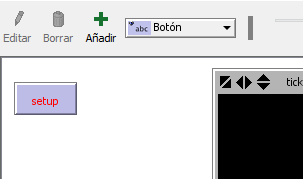
\includegraphics[width=8cm, height=5cm]{./imagenes/image1.png}
\end{figure}


\item Si desea ver el actual mensaje de error, haga clic en el botón.
\item Ahora vamos a crear el procedimiento "setup", de modo que el mensaje de error desaparecerá:
\item Cambiese a la pestaña Procedures.
\item Escriba lo siguiente:


\begin{lstlisting}
to setup
   clear-all
   create-turtles 100
   ask turtles[ setxy random-xcor random-ycor]
end
\end{lstlisting}


Tenga en cuenta que las líneas tienen diferentes sangrías. La mayoría de las personas encuentra útil sangrar su código como en este, sin embargo no es obligatorio. Esto hace más fácil leer y cambiar el código. Su procedimiento inició con la palabra to y terminó con la palabra end. Cada nuevo procedimiento que cree comenzará y terminará con estas dos palabras.


\begin{center}
	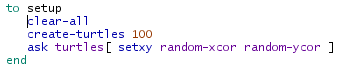
\includegraphics[width=8cm]{./imagenes/image2.png}
\end{center}

\item Cuando haya terminado de escribir cambie a la interfaz y presione el botón setup que hizo anteriormente. Verá las tortugas dispersas alrededor del mundo:


\begin{center}
	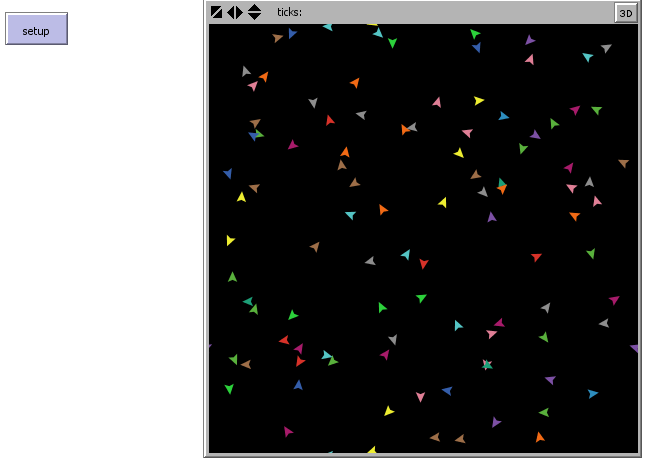
\includegraphics[width=8cm]{./imagenes/image3.png}
\end{center}


\begin{center}
	Haciendo el botón go
\end{center}

Ahora haga un botón llamado "go". Siga los mismos pasos que utilizó para hacer el botón setup, excepto:

\item En Commands introduzca go en lugar de setup.
\item Marque  "forever" en la casilla de verificación del diálogo de edición.

\begin{center}
	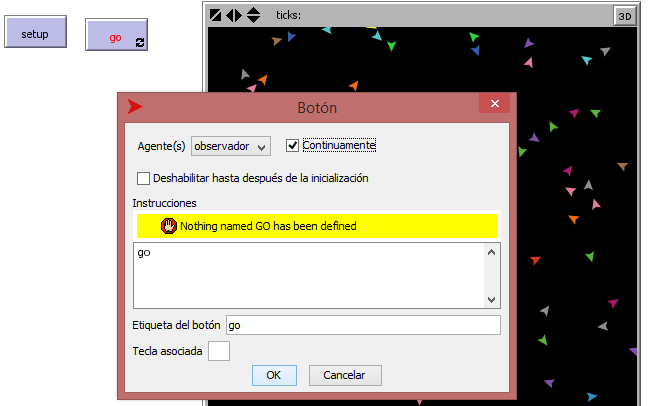
\includegraphics[width=8cm]{./imagenes/image4.png}
\end{center}

\item A continuación, agregue un procedimiento Go en la pestaña de procedimientos (Procedures):

\begin{lstlisting}
 to go
    move-turtles
 end
\end{lstlisting}

\item Agregue el procedimiento move-turtles después del procedimiento go:

\begin{lstlisting}
to go
   move-turtles
 end

to move-turtles
	ask turtles[
       	right random 360
       	forward 1
	]
end
\end{lstlisting}

\begin{center}
		PARCHES Y VARIABLES
\end{center}

\item Regresemos al procedimiento setup. Podemos reescribirlo de la siguiente manera:

\begin{lstlisting}
to setup
    clear-all
    setup-patches
    setup-turtles
end
\end{lstlisting}

\item La nueva definición de setup se refiere a dos nuevos procedimientos. Para definir setup-patches añada lo siguiente:

\begin{lstlisting}
 to setup-patches
    ask patches [ set pcolor green ]
 end
\end{lstlisting}

El procedimiento setup-patch establece en verde el color de cada parche al comenzar. (La variable del color de la tortuga es color; la del parche es pcolor.)

La única parte que permanecen en nuestro nuevo 'setup' que aún está indefinida es setup-turtles.

\item Añada también este procedimiento:
\begin{lstlisting}
 to setup-turtles
    create-turtles 100
    ask turtles [ setxy random-xcor random-ycor ]
 end
\end{lstlisting}

¿Advirtió que el nuevo procedimiento setup-turtles tiene la mayoría de los mismos comandos que el antiguo procedimiento setup?

\begin{center}
	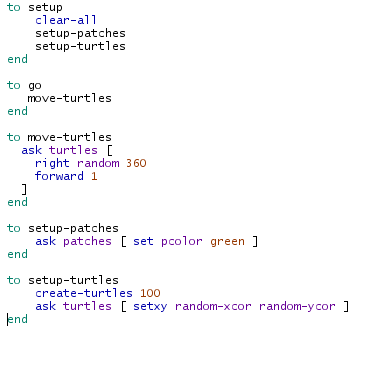
\includegraphics[width=8cm]{./imagenes/image5.png}
\end{center}


\item Vuelva a la pestaña de Interfaz.
\item Pulse el botón setup.

Voila! Aparece un exuberante paisaje NetLogo completo con las tortugas y los parches verdes:

\begin{center}
	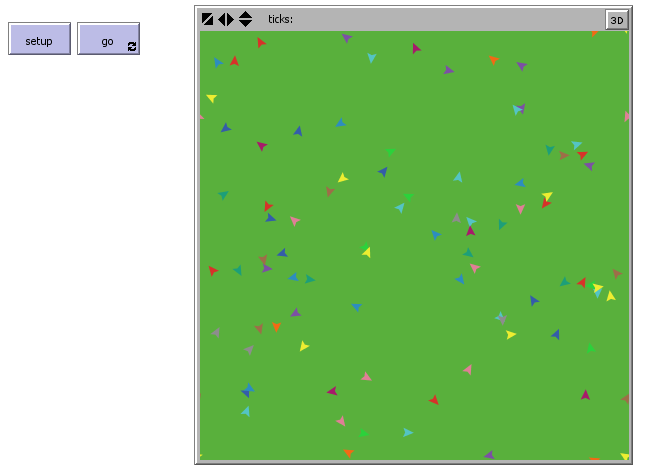
\includegraphics[width=8cm]{./imagenes/image6.png}
\end{center}


\begin{center}
VARIABLES DE TORTUGA	
\end{center}

De modo que tenemos algunas tortugas corriendo en un paisaje, pero nada están haciendo con ello. Vamos a añadir algo de interacción entre las tortugas y los parches.

Haremos a las tortugas comer "pasto" (los parches verdes), reproducirse y morir. La hierba crecerá gradualmente después de ser comida.

Necesitamos una manera de controlar cuando una tortuga se reproduce y cuándo muere. Vamos a determinarlo haciendo el seguimiento de la cantidad de "energía" que tiene cada una de las tortugas. Para hacer esto necesitamos añadir una nueva variable en la tortuga.

Ya ha visto la construcción de variables de la tortuga tales como color. Para crear una nueva variable de la tortuga, añadimos una declaración turtles-own   (tortugas-propia) en la parte superior de la pestaña de procedimientos, antes que todos los procedimientos. Llamela energy (energía):

\begin{lstlisting}
turtles-own [energy] 

to go
   move-turtles
   eat-grass
end

\end{lstlisting}

Vamos a utilizar esta recientemente definida variable (energy) para permitirle a las tortugas comer.

\item Cambie a la pestaña de Procedimientos.
\item Reescriba el procedimiento go de la siguiente manera:

\begin{lstlisting}
to go
   move-turtles
   eat-grass
end
\end{lstlisting}

\item Agrega el nuevo procedimiento eat-grass (comer-pasto):

\begin{lstlisting}
to eat-grass
   ask turtles [
      if pcolor = green [
         set pcolor black
      set energy (energy + 10) ] 
   ] 
end
\end{lstlisting}


A continuación vamos a hacer que el movimiento de las tortugas utilice un poco de la energía de las tortugas.

\item Reescriba move-turtles así:

\begin{lstlisting}
to move-turtles
   ask turtles [
      right random 360
      forward 1
	  set energy (energy - 1)
   ] 
end
\end{lstlisting}

En la medida en que cada tortuga deambula pierde una unidad de energía a cada paso.

Ahora vaya a la interfaz y presione el botón setup y luego el botón go, verá los parches volverse negros a medida que las tortugas viajan sobre ellos.

\begin{center}
	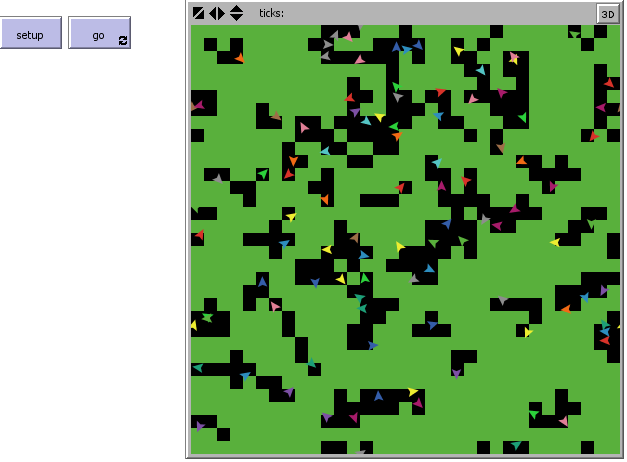
\includegraphics[width=8cm]{./imagenes/image7.png}
\end{center}


\begin{center}
	 MONITORES
\end{center}

A continuación creará en la interfaz dos monitores con la barra de herramientas. (Usted los hace tal como a los controles deslizantes (sliders) y a los botones, usando el icono del monitor de la barra de herramientas.) Vamos a hacer ahora el primer monitor.


\item Cree un monitor, utilizando el icono del monitor de la barra de herramientas,  haga clic en un lugar abierto de la interfaz.
\item Aparecerá un cuadro de diálogo.
\item En el cuadro de diálogo escriba: count turtles (contar las tortugas, ver imagen inferior).
\item Pulse el botón OK para cerrar el cuadro de diálogo.

\begin{center}
	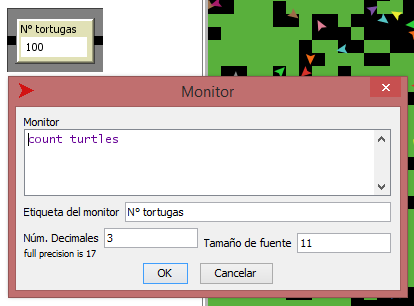
\includegraphics[width=8cm]{./imagenes/image8.png}
\end{center}

Vamos a hacer ahora el segundo monitor:

\item Cree un monitor, utilizando el icono del monitor de la barra de herramientas y haga clic en un lugar abierto de la interfaz.

Aparecerá un cuadro de diálogo.

\item En la sección Reportero del cuadro de diálogo escriba: count patches with [pcolor = green]  (ver imagen inferior).
\item En la sección Display name del cuadro de diálogo escriba: green patches


Pulse el botón OK para cerrar el cuadro de diálogo.


\begin{center}
	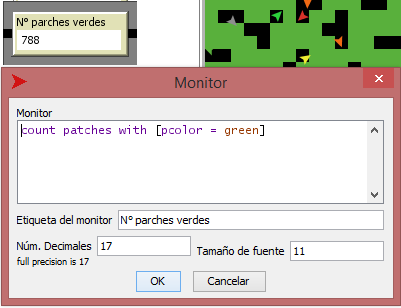
\includegraphics[width=8cm]{./imagenes/image9.png}
\end{center}


\begin{center}
INTERRUPTORES Y ETIQUETAS
\end{center}

\item Para crear un interruptor, haga clic en el interruptor de la barra de herramientas (en la pestaña Interfaz) y haga clic en un punto abierto en la interfaz.

Aparecerá un cuadro de diálogo.

\item En la sección de variable Global del cuadro de diálogo escriba: show-energy? No olvide de incluir el signo de interrogación en el nombre. (Vea la imagen a continuación.)

\begin{lstlisting}
to eat-grass
    ask turtles [
 		if pcolor = green [
		set pcolor black
    	set energy (energy + 10)
    	] 
    	ifelse show-energy?
       		[ set label energy ]
 		[ set label "" ]
    ] 
end
\end{lstlisting}


Cuando el interruptor está encendido, verá la energía de cada tortuga incrementarse cada vez que come hierba. También verá su energía disminuir cada vez que se mueve.


\begin{center}
	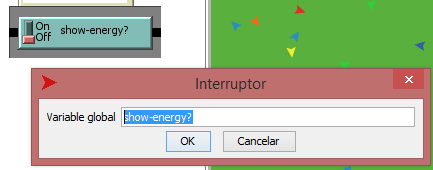
\includegraphics[width=8cm]{./imagenes/image10.png}
\end{center}

\begin{center}
 MAS PROCEDIMIENTOS
\end{center}

Ahora nuestro tortugas están comiendo; vamos a hacer que también se reproduzcan y mueran. Además vamos a hacer que la hierba rebrote. Ahora mismo vamos a añadir estos tres comportamientos haciendo tres procedimientos separados. Uno para cada comportamiento.


\item Vaya a la pestaña de procedimientos (Procedures).
\item Reescribir el procedimiento go de la siguiente manera:
\begin{lstlisting}
to go
    move-turtles
    eat-grass
    reproduce
    check-death
    regrow-grass 
 end
\end{lstlisting} 
 
\item Añada los procedimientos para reproduce, check-death y regrow-grass, como se indica a continuación:
 
\begin{lstlisting} 
 to reproduce ;; reproducirse
    ask turtles [
       if energy > 50 [
            set energy energy - 50
             hatch 1 [ set energy 50 ]
          ] 
       ] 
 end

 to check-death ;; verificar muerte
      ask turtles [
          if energy <= 0 [ die ]
       ] 
 end

 to regrow-grass ;; rebrotar pasto
    ask patches [
       if random 100 < 3 [ set pcolor green ]
       ] 
 end
\end{lstlisting}

\item Vaya a la Interfaz y presione los botones setup y go.


\begin{center}
	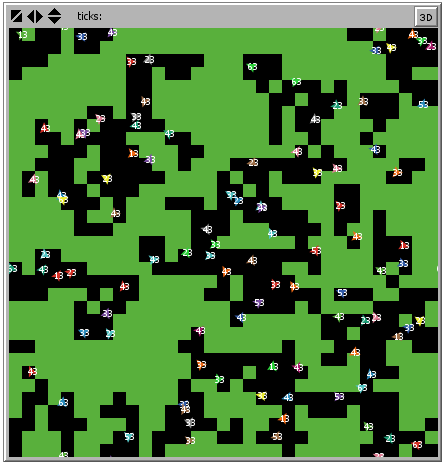
\includegraphics[width=8cm]{./imagenes/image11.png}
\end{center}

\paragraph{Observación}Las tortugas ahora mueren y se reproducen, además el pasto vuelve a crecer.

\begin{center}
GRAFICACIÓN
\end{center}

\item Cambiemos setup para llamar al nuevo procedimiento, do-plots (hacer gráficas), que estamos a punto de añadir:
 \begin{lstlisting}
 to setup
    clear-all
    setup-patches
    setup-turtles
    do-plots
 end
\end{lstlisting}
\item Además, cambiemos go para llamar al procedimiento do-plots:
\begin{lstlisting}
to go
    move-turtles
    eat-grass
    reproduce
    check-death
   regrow-grass 
    do-plots
 end
 \end{lstlisting}
\item Ahora agregue el nuevo procedimiento. Lo que estamos graficando será el número de tortugas y el número de parches verdes contra el tiempo. En cada paso de tiempo (una ejecución simple a través del procedimiento go) estos valores se añaden a la gráfica.
\begin{lstlisting}
to do-plots
    set-current-plot "Totals"
    set-current-plot-pen "turtles"
    plot count turtles
    set-current-plot-pen "grass"
    plot count patches with [pcolor = green]
 end
\end{lstlisting}
\item Cree un gráfico, utilizando el icono plot de la barra de herramientas y haga clic en un lugar abierto en la interfaz.
\item Establezca su nombre como "Totals" (ver imagen inferior)
\item Establezca el eje de las X con la etiqueta "time"
\item Establezca el eje Y con etiqueta "total"

\begin{center}
	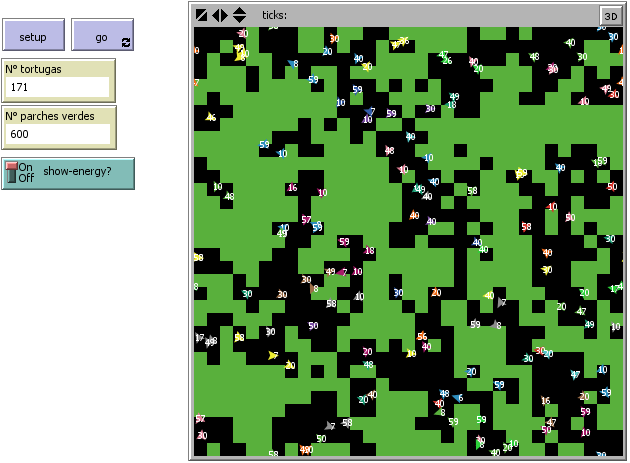
\includegraphics[width=8cm]{./imagenes/image12.png}
\end{center}

\item Con el cuadro de diálogo de Plot (Gráfica) aun abierto, pulse el botón 'Create' en el diálogo de Plot para crear una nueva curva.
\item Introduzca el nombre de esta curva como "turtles" y pulse OK en el diálogo de "Enter Pen Name". (ver imagen inferior)
\item Pulse nuevamente el botón 'Crear' en el cuadro de diálogo de nuevo, para crear una segunda curva nueva.
\item Introduzca el nombre de esta curva como "grass" y pulse OK en el cuadro de diálogo "Enter Pen Name". (ver imagen inferior)
\item Seleccione el color de la curva y cámbielo a verde.
\item Seleccione OK en el cuadro de diálogo de la Plot (Gráfica).

\begin{center}
	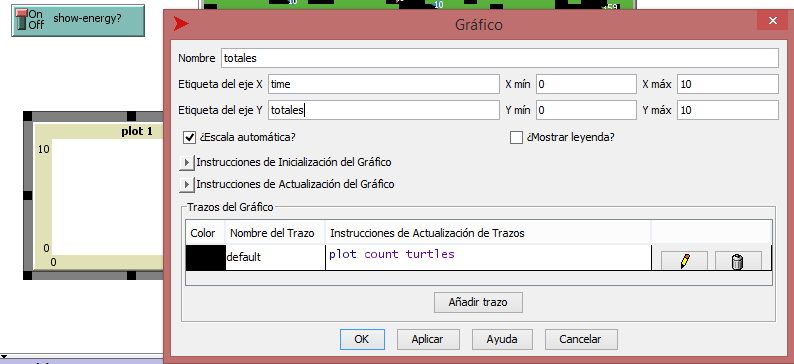
\includegraphics[width=8cm]{./imagenes/image13.png}
\end{center}

\begin{center}
CONTADOR DE TICS
\end{center}

\item Cambie el procedimiento go:

\begin{lstlisting}
 to go
    if ticks >= 500 [ stop ]
    move-turtles 
    eat-grass
    reproduce
    check-death
   regrow-grass 
    tick 
    do-plots 
 end 
\end{lstlisting} 

\item Ahora configure y ejecute el modelo.

\begin{center}
	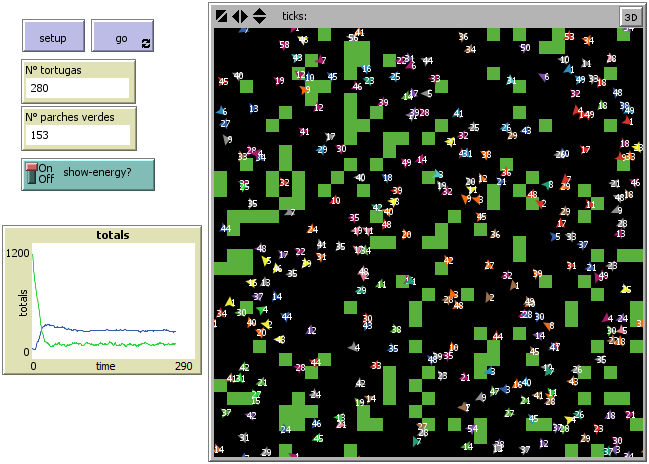
\includegraphics[width=8cm]{./imagenes/image14.png}
\end{center}

\begin{center}
ALGUNOS DETALLES ADICIONALES
\end{center}

\item Cree una variable slider llamada "numero" usando el ícono monitor de la barra de herramientas y haga clic en un lugar limpio de la interfaz. Intente cambiando los valores mínimo y máximo en el slider.
\item Luego, dentro de setup-turtles, en lugar de create-turtles 100 usted puede escribir:

\begin{lstlisting}
 to setup-turtles
    create-turtles number
    ask turtles [ setxy random-xcor random-ycor ]
 end
\end{lstlisting}
\item Y dentro de reproduce haga este cambio:
\begin{lstlisting}
to reproduce
    ask turtles [
       if energy > birth-energy [
          set energy energy - birth-energy
          hatch 1 [ set energy birth-energy ]
         ] 
    ] 
 end
\end{lstlisting}


\begin{center}
	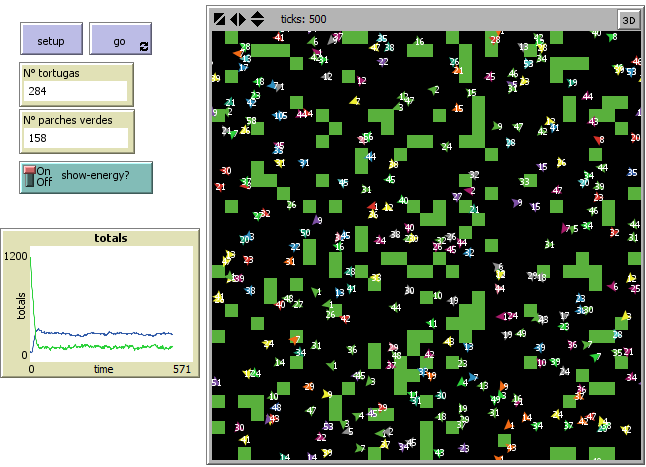
\includegraphics[width=8cm]{./imagenes/image15.png}
\end{center}


\begin{center}
	EL CODIGO COMPLETO DE LA SIMULACIÓN
\end{center}

\begin{lstlisting}
turtles-own [energy] 

 to setup
    clear-all
    setup-patches
    setup-turtles
    do-plots
    reset-ticks
end

to go
    if ticks >= 500 [ stop ]
    move-turtles 
    eat-grass
    reproduce
    check-death
    regrow-grass 
    tick 
    do-plots 
end 

to move-turtles
    ask turtles [
       right random 360
       forward 1
    set energy energy - 1 ] 
end

to setup-patches
    ask patches [ set pcolor green ]
end

 to setup-turtles
    create-turtles number
    ask turtles [ setxy random-xcor random-ycor ]
end

to eat-grass
  ask turtles [
    if pcolor = green [
      set pcolor black
      set energy (energy + 10)
    ] 
    ifelse show-energy?
    [ set label energy ]
    [ set label "" ]
  ] 
end

to reproduce
  ask turtles [
    if energy > birth-energy [
      set energy energy - birth-energy
      hatch 1 [ set energy birth-energy ]
    ] 
  ]
end


to check-death ;; verificar muerte
  ask turtles [
    if energy <= 0 [ die ]
  ] 
end

to regrow-grass ;; rebrotar pasto
  ask patches [
    if random 100 < 3 [ set pcolor green ]
  ] 
end


to do-plots
    set-current-plot "Totals"
    set-current-plot-pen "turtles"
    plot count turtles
    set-current-plot-pen "grass"
    plot count patches with [pcolor = green]
end

\end{lstlisting}



\end{itemize}


\end{document}